\chapter{TDT4295 - Computer Design Project}
\label{sec:intro}

The Computer Design Project is held at NTNU every fall.
It is a large, project-based subject in which students create a working computing platform, more or less from scratch.
This year saw high enough participation that two assignments were presented, and two groups formed around these.
This report details the work done and solution implemented by the vector graphics processor group.

\section{Assignment}

This years assignment focuses on graphics, exploring both of the traditional ways of representing and processing graphics; raster-based and vector-based.
Two distinct assignment texts were presented by the course staff, one focusing on raster-based graphics, the other on vector graphics.
The following is a verbatim copy of the vector graphics assignment text \cite{assignment-text}.

\subsection{Assignment Text - A Vector Graphics Processor}

Image generation using vector graphics as the core method is a powerful and scalable way of generating image data.
Vector graphics represents images at a higher abstraction level than single-pixels.
A vector graphics processor can make use of drawing instructions to produce images, which is a task well suited for hardware acceleration \cite{openvg}.
Parallelization with multiple cores and/or at the instruction level are architectural possibilities that can be exploited to design a specialized processor.
The task is to design and implement a processor for producing vector graphics.
Figure \ref{fig:vector-display-network-analyzer} illustrates a vector display which takes in vector drawing commands (instead of a stream of pixels) as input.

\begin{figure}[h!]
    \centering
    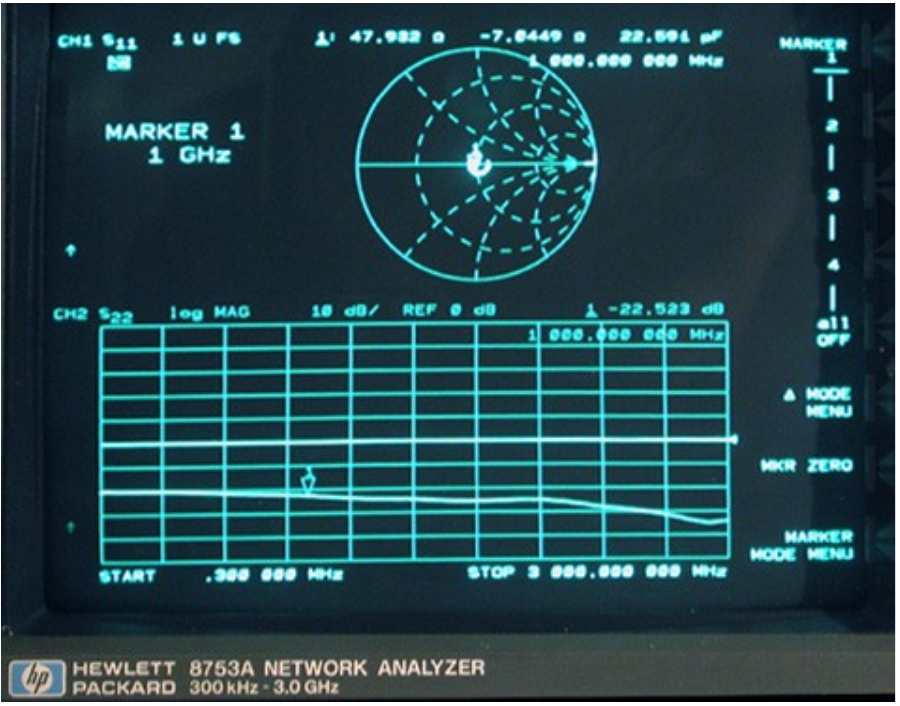
\includegraphics[width=0.8\linewidth]{images/network-analyzer-vector-graphics-display.png}
    \caption{A vector graphics display on a network analyzer\cite{assignment-text}.}
    \label{fig:vector-display-network-analyzer}
\end{figure}

\section{Vector Graphics - A Short Introduction}

Vector graphics expresses the contents of an image mathematically.
A line is defined by its endpoints, a square as the bounding box of two points and curves by the position of their controlpoints.
These points are relative to the coordinate system of a scene, an abstract represantation of an image.
A scene is not tied to any specific physical screen resolution, but can be scaled to fit any resolution without loss of detail.

The major advantages of vector graphics are expressiveness and scalability.
Modern computing devices come in many sizes and aspect ratios.
With raster based solutions, graphics have to be regenerated for each new display size.
A vector based solution is inherently resolution independent, allowing for asset reuse across devices.

\section{A Vector Graphics Computer Architecture}

The group chose to make a general purpose computer with support for producing and processing vector graphics.
The computer would read instructions from memory, execute them on a processor core and render vector based scenes to different outputs.
Since most commonly available display devices expect raster based input, an oscilloscope was chosen as the primary output device, HDMI as a secondary.
As a whole, the system should be assembled on a custom PCB, with the microcontroller serving as an I/O-unit while the main processor architecture and output-modules should be implemented on the FPGA.

\section{Requirements}

The group decided on a set of functional requirements based on our initial research. These are listed in table \ref{tbl:func_req}.
Non-functional requirements given in the assignment text are listed in list \ref{lst:non_func_req}.

\begin{table}[h!]
    \begin{tabular}{|l|l|}
        \hline
        Requirement                                                             & Priority \\ \hline
        The system should be able to produce and process vector primitives      & High     \\ \hline
        The system should display primitives on an oscilloscope                 & High     \\ \hline
        The system should support both straight lines and general bezier curves & High     \\ \hline
        The processor should be general                                         & High     \\ \hline
        The system should support modification of primitives                    & Medium   \\ \hline
        The system should rasterize primitives and support HDMI as an output    & Medium   \\ \hline
        A toolchain supporting the system should be available                   & Low      \\ \hline
    \end{tabular}
    \caption{Functional requirements.}
    \label{tbl:func_req}
\end{table}

//TODO: Should this be a figure?
\begin{figure}[h!]
\begin{itemize}
        \item The processor should be implemented on a Xilinx FPGA.
        \item The unit must utilize a Silicon Labs EFM32 microcontroller as an I/O processor.
        \item The budget of 10 000 NOK should cover components and PCB production.
\end{itemize}
        \label{lst:non_func_req}
        \caption{Non-functional requirements.}
\end{figure}

\section{About this report}

This report is meant to give a thorough understanding of the architecture designed by the group,
Having introduced the assignment, the next chapters will introduce the system created by the group as well as give some background on computer graphics and a theoretical overview of vector graphics.


Part two presents the designed architecture in detail, outlines the programming model and elaborates on the implementation of specific subparts of the system.
Finally, part three presents performed tests, results, discussion and a conclusion.


\section{Lab Environment}
The NTNU Computer Design Lab was used frequently for this project. The lab contains a wide variety of oscillators, signal generators and logic analyzers, which was used to test different parts of the system. The lab also contains soldering equipment and aids - which was used extensively by the team when soldering the PCB - as well as loads of assorted electronic components.

Another lab at NTNU, nicknamed "sauna", was used by the team when programming the solution. This includes computers running Ubuntu, and has tools for working with FPGAs from Xilinx installed. This lab is also used in the Computer Design course.

\section{Terminology}
// TODO: Describe any conventions used in the report. E.g. using "the group" for everyone and "the team" for the different task groups (PCB team, I/O team etc.)